% Schematic of inverse Thomson scattering (head-on relativistic collision).
% Left panel: before collision (relativistic electron moving right, red laser photon moving left).
% Right panel: after collision (electron continues right with slightly lower energy,
% backscattered high-frequency X-ray photon moves right ahead of the electron).
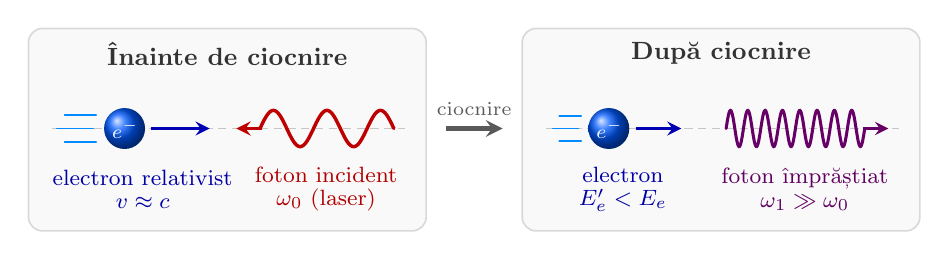
\begin{tikzpicture}[>=stealth, font=\footnotesize]
  % ==========================================================================
  % Left panel: Before collision
  % ==========================================================================
  \filldraw[fill=gray!5, draw=gray!30, rounded corners=5pt, line width=0.6pt]
    (-0.10, -1.25) rectangle (4.95, 1.32);

  \node[black!80, font=\small\bfseries] at (2.425, 1.00) {Înainte de ciocnire};

  % Collision axis
  \draw[gray!45, densely dashed, line width=0.5pt] (0.20, 0.05) -- (4.68, 0.05);

  % Speed lines behind relativistic electron
  \draw[blue!45!cyan, line width=0.7pt, line cap=round] (0.36, 0.22) -- (0.76, 0.22);
  \draw[blue!45!cyan, line width=0.7pt, line cap=round] (0.26, 0.05) -- (0.72, 0.05);
  \draw[blue!45!cyan, line width=0.7pt, line cap=round] (0.36, -0.12) -- (0.76, -0.12);

  % Relativistic electron
  \shade[ball color=blue!65!cyan] (1.12, 0.05) circle (0.26);
  \node[white, font=\scriptsize\bfseries] at (1.13, 0.04) {$e^-$};
  \draw[->, very thick, blue!70!black] (1.46, 0.05) -- (2.20, 0.05);

  \node[blue!65!black, align=center] at (1.35, -0.72) {electron relativist\\[-1pt]$v \approx c$};

  % Incident low-frequency laser photon (red, long wavelength, travelling left)
  \draw[red!75!black, line width=1.25pt, line cap=round,
    domain=2.84:4.54, samples=120, variable=\x, smooth]
    plot (\x, {0.05 + 0.23*sin(deg(2*pi*(\x - 2.84)/0.68))});
  \draw[->, red!75!black, line width=1.25pt] (2.86, 0.05) -- (2.54, 0.05);

  \node[red!70!black, align=center] at (3.68, -0.72) {foton incident\\[-1pt]$\omega_0$ (laser)};

  % ==========================================================================
  % Center transition arrow
  % ==========================================================================
  \draw[->, line width=1.6pt, black!65] (5.20, 0.05) -- (5.92, 0.05);
  \node[black!65, font=\scriptsize] at (5.56, 0.30) {ciocnire};

  % ==========================================================================
  % Right panel: After collision
  % ==========================================================================
  \filldraw[fill=gray!5, draw=gray!30, rounded corners=5pt, line width=0.6pt]
    (6.17, -1.25) rectangle (11.22, 1.32);

  \node[black!80, font=\small\bfseries] at (8.695, 1.00) {După ciocnire};

  % Collision axis
  \draw[gray!45, densely dashed, line width=0.5pt] (6.47, 0.05) -- (10.95, 0.05);

  % Speed lines behind electron (slightly shorter)
  \draw[blue!45!cyan, line width=0.65pt, line cap=round] (6.64, 0.21) -- (6.92, 0.21);
  \draw[blue!45!cyan, line width=0.65pt, line cap=round] (6.56, 0.05) -- (6.88, 0.05);
  \draw[blue!45!cyan, line width=0.65pt, line cap=round] (6.64, -0.11) -- (6.92, -0.11);

  % Electron after collision
  \shade[ball color=blue!65!cyan] (7.27, 0.05) circle (0.26);
  \node[white, font=\scriptsize\bfseries] at (7.28, 0.04) {$e^-$};
  \draw[->, very thick, blue!70!black] (7.61, 0.05) -- (8.19, 0.05);

  \node[blue!65!black, align=center] at (7.45, -0.72) {electron\\[-1pt]$E_e' < E_e$};

  % Scattered high-frequency photon (violet, short wavelength, travelling right)
  \draw[violet!80!black, line width=1.1pt, line cap=round,
    domain=8.76:10.52, samples=260, variable=\x, smooth]
    plot (\x, {0.05 + 0.23*sin(deg(2*pi*(\x - 8.76)/0.22))});
  \draw[->, violet!80!black, line width=1.1pt] (10.50, 0.05) -- (10.82, 0.05);

  \node[violet!75!black, align=center] at (9.76, -0.72) {foton împrăștiat\\[-1pt]$\omega_1 \gg \omega_0$};
\end{tikzpicture}
